%%
%% This is file `sample-manuscript.tex',
%% generated with the docstrip utility.
%%
%% The original source files were:
%%
%% samples.dtx  (with options: `all,proceedings,bibtex,manuscript')
%% 
%% IMPORTANT NOTICE:
%% 
%% For the copyright see the source file.
%% 
%% Any modified versions of this file must be renamed
%% with new filenames distinct from sample-manuscript.tex.
%% 
%% For distribution of the original source see the terms
%% for copying and modification in the file samples.dtx.
%% 
%% This generated file may be distributed as long as the
%% original source files, as listed above, are part of the
%% same distribution. (The sources need not necessarily be
%% in the same archive or directory.)
%%
%%
%% Commands for TeXCount
%TC:macro \cite [option:text,text]
%TC:macro \citep [option:text,text]
%TC:macro \citet [option:text,text]
%TC:envir table 0 1
%TC:envir table* 0 1
%TC:envir tabular [ignore] word
%TC:envir displaymath 0 word
%TC:envir math 0 word
%TC:envir comment 0 0
%%
%% The first command in your LaTeX source must be the \documentclass
%% command.
%%
%% For submission and review of your manuscript please change the
%% command to \documentclass[manuscript, screen, review]{acmart}.
%%
%% When submitting camera ready or to TAPS, please change the command
%% to \documentclass[sigconf]{acmart} or whichever template is required
%% for your publication.
%%
%%
\documentclass[acmsmall,nonacm]{acmart}
%%
%% \BibTeX command to typeset BibTeX logo in the docs
\AtBeginDocument{%
  \providecommand\BibTeX{{%
    Bib\TeX}}}

\settopmatter{printacmref=false} % removes ACM reference format block
\renewcommand\footnotetextcopyrightpermission[1]{} % removes copyright footnote
\pagestyle{plain} % optional: removes fancy headers

\onecolumn
    

%% Rights management information.  This information is sent to you
%% when you complete the rights form.  These commands have SAMPLE
%% values in them; it is your responsibility as an author to replace
%% the commands and values with those provided to you when you
%% complete the rights form.
\setcopyright{acmlicensed}
\copyrightyear{2025}
\acmYear{2025}
\acmDOI{XXXXXXX.XXXXXXX}
%% These commands are for a PROCEEDINGS abstract or paper.
\acmConference[Conference acronym 'XX]{N/A}{Jun 2025 - Dec 2025}{Woodstock, NY}
%%
%%  Uncomment \acmBooktitle if the title of the proceedings is different
%%  from ``Proceedings of ...''!
%%
%%\acmBooktitle{Woodstock '18: ACM Symposium on Neural Gaze Detection,
%%  June 03--05, 2018, Woodstock, NY}
\acmISBN{978-1-4503-XXXX-X/2018/06}


%%
%% Submission ID.
%% Use this when submitting an article to a sponsored event. You'll
%% receive a unique submission ID from the organizers
%% of the event, and this ID should be used as the parameter to this command.
%%\acmSubmissionID{123-A56-BU3}

%%
%% For managing citations, it is recommended to use bibliography
%% files in BibTeX format.
%%
%% You can then either use BibTeX with the ACM-Reference-Format style,
%% or BibLaTeX with the acmnumeric or acmauthoryear sytles, that include
%% support for advanced citation of software artefact from the
%% biblatex-software package, also separately available on CTAN.
%%
%% Look at the sample-*-biblatex.tex files for templates showcasing
%% the biblatex styles.
%%

%%
%% The majority of ACM publications use numbered citations and
%% references.  The command \citestyle{authoryear} switches to the
%% "author year" style.
%%
%% If you are preparing content for an event
%% sponsored by ACM SIGGRAPH, you must use the "author year" style of
%% citations and references.
%% Uncommenting
%% the next command will enable that style.
%%\citestyle{acmauthoryear}


%%
%% end of the preamble, start of the body of the document source.
\usepackage{amssymb}
\usepackage{amsmath}
\newcommand{\overbar}[1]{\mkern 1.5mu\overline{\mkern-1.5mu#1\mkern-1.5mu}\mkern 1.5mu}

% --- Safe cross-engine definition for \bo ---
\usepackage{iftex}

\ifPDFTeX
  \DeclareRobustCommand{\bo}{\mathfrak{B}}
\else
  \usepackage{fontspec}
  \newfontfamily{\vaifont}{Noto Sans Vai}

  % helper to typeset the glyph in text at the current math size
  \newcommand{\vaibo}[1]{{\vaifont #1}}

  \DeclareRobustCommand{\bo}{%
    \ifmmode
      \mathchoice
        {\text{\vaibo{ꕸ}}}            % displaystyle
        {\text{\vaibo{ꕸ}}}            % textstyle
        {\scriptstyle\text{\vaibo{ꕸ}}}% scriptstyle
        {\scriptscriptstyle\text{\vaibo{ꕸ}}}% scriptscriptstyle
    \else
      {\vaibo{ꕸ}}%
    \fi
  }
\fi

\newcommand{\bfa}{\bo}

\usepackage{subcaption}
\usepackage{tikz}

\usepackage[colorinlistoftodos]{todonotes}

% Define author-specific todos
\newcommand{\liam}[1]{\todo[inline, color=blue!40]{\begin{minipage}{\textwidth-4pt}\textbf{[Liam Monninger]:} #1\end{minipage}}}
\usetikzlibrary{cd}

\begin{document}

%%
%% The "title" command has an optional parameter,
%% allowing the author to define a "short title" to be used in page headers.
\title{Byzantine Fault Allowing Protocols}

%%
%% The "author" command and its associated commands are used to define
%% the authors and their affiliations.
%% Of note is the shared affiliation of the first two authors, and the
%% "authornote" and "authornotemark" commands
%% used to denote shared contribution to the research.
\author{Liam Monninger}
\email{liam@ramate.io}
\affiliation{%
  \institution{Ramate LLC}
  \city{Durham}
  \state{California}
  \country{USA}
}

%%
%% By default, the full list of authors will be used in the page
%% headers. Often, this list is too long, and will overlap
%% other information printed in the page headers. This command allows
%% the author to define a more concise list
%% of authors' names for this purpose.
\renewcommand{\shortauthors}{Monninger}

%%
%% The abstract is a short summary of the work to be presented in the
%% article.
\begin{abstract}
    I've written this memo to describe to friends and colleagues the beginning of my study of a category of distributed computing protocols which I call Byzantine Fault Allowing. I begin with the motivation for the study. I then provide a trivial combinatorial example of a protocol assumed to be in the category. Finally, I suggest more abstract constructions with which the study is properly concerned.

    Most terms and notation follow [HKR]. The final section introduces provisional and more suggestive terms. 
\end{abstract}

%%
%% The code below is generated by the tool at http://dl.acm.org/ccs.cfm.
%% Please copy and paste the code instead of the example below.
%%
\begin{CCSXML}
<ccs2012>
 <concept>
  <concept_id>00000000.0000000.0000000</concept_id>
  <concept_desc>Do Not Use This Code, Generate the Correct Terms for Your Paper</concept_desc>
  <concept_significance>500</concept_significance>
 </concept>
 </concept>
</ccs2012>
\end{CCSXML}

\ccsdesc[500]{Do Not Use This Code~Generate the Correct Terms for Your Paper}
\ccsdesc[300]{Do Not Use This Code~Generate the Correct Terms for Your Paper}
\ccsdesc{Do Not Use This Code~Generate the Correct Terms for Your Paper}
\ccsdesc[100]{Do Not Use This Code~Generate the Correct Terms for Your Paper}

%%
%% Keywords. The author(s) should pick words that accurately describe
%% the work being presented. Separate the keywords with commas.
\keywords{Byzantine Fault Allowing, Byzantine Fault Tolerance, State Machine Replication, Byzantine Fault Tolerant Systems}

\received{12 January 2026}
\received[revised]{12 January 2026}
\received[accepted]{12 January 2026}

%%
%% This command processes the author and affiliation and title
%% information and builds the first part of the formatted document.
\maketitle

\section{Introduction}

\subsection{Academia}

\subsection{Industry}

\section{Motivation}
To motivate the category $\bfa$, we perform a series of exercises. First, we consider a Byzantine majority algorithm, denoted $B$, as a lossless expert model, representing a prospective fixed-point in $\bfa$. Next, we consider combinatorial parameterizations of $B$, providing some initial morphisms on members of $\bfa$. Finally, we examine a topological approximation of $B$, as an indication of non-trivial morphisms in $\bfa$.

\subsection{Expert Models, Byzantine Majorities, and $B$}
To begin motivating structures of $\bfa$, we argue that coordinating state machine replicas presents an online decision problem for which Byzantine majority presents a lossless expert model.

First, consider the information available in a state machine replica protocol. We know the following:

\begin{itemize}
    \item There exists a set of replicas $P$ which has disjoint subsets $H$ and $F$ such that $H \cap F = \emptyset$ and $H \cup F = P$.
    \item A client of the system will be able to obtain certificates of computed state transitions $r' \in R'$ from the replicas. We will denote these as $Q: R' \to 2^P$. Note that the value of $Val(Q(r')) = r'$ for all $r' \in R'$.
    \item To be a member of a quorum $Q(r')$, a replica must compute and broadcast the value $r'$.
    \item Honest nodes compute a correct state transition. Tautologically, a state transition is correct if the quorum of which it is a member intersects with the honest set $Q(r') \cap H \neq \emptyset$.
\end{itemize}

Now consider our objectives. We want:

\begin{itemize}
    \item Our state transition is correct. 
    \item Our state transition is consistent, i.e., records the past effects of previous state transitions.
\end{itemize}

Our determination for correctness $Cor$ is given to us by our tautology above:

\begin{flalign*}
&Cor(r') \triangleq (Q(r') \cap H \neq \emptyset) \\
\end{flalign*}

Consistency is less obvious. For the purpose of this motivation, we will assume a sequence of state transitions $r'_1, r'_2, \cdots, r'_n$ which we will denote as $R'$. We will say that a quorum $Q(r'_j)$ is consistent if and only if its predecessor $Q(r'_{j-1})$ is consistent and the two quora intersect, i.e., $Q(r'_j) \cap Q(r'_{j-1}) \neq \emptyset$. Observe that the expansion of our consistency function $Con$ records all the effects of previous state transitions satisfying our original semantic intent:

\begin{flalign*}
  &C(r'_i, r'_j) \triangleq (Q(r'_i) \cap Q(r'_j) \neq \emptyset) \\
  &Con(r'_j) = Con(r'_{j-1}) \land C(r'_{j-1}, r'_j) \\
  &\quad = C(r'_0, r'_1) \land \cdots \land  C(r'_{j-1}, r'_j) \\
\end{flalign*}

We combine these definitions of correctness and consistency to form our objective $Obj$. Observe that the expansion records all correct effects of previous state transitions satisfying the original semantic intent:

\begin{flalign*}
  &O(r'_i, r'_j) \triangleq (Q(r'_i) \cap Q(r'_j) \cap H \neq \emptyset) \\
  &Obj(r'_j) = Obj(r'_{j-1}) \land O(r'_{j-1}, r'_j) \\
  &\quad = Obj(r'_0) \land O(r'_0, r'_1) \land \cdots \land O(r'_{j-1}, r'_j) \\
  &\quad = Obj(r'_0)\\
  &\qquad \land (Q(r'_0) \cap Q(r'_1) \cap H \neq \emptyset)\\
  &\qquad \cdots\\
  &\qquad \land (Q(r'_{j-1}) \cap Q(r'_j) \cap H \neq \emptyset)\\
\end{flalign*}

We transform this into a loss function $Loss$ which counts the number of incorrect or inconsistent quora for our expert model as below. Note that later we will discuss alternative definitions of loss:

\begin{flalign*}
  &Loss(r'_j) = \\
  &\quad \sum_{r'_i \in [r'_0, r'_j]} [\neg Obj(r'_i) ] \\
  &\quad = [\neg Obj(r'_0)] + [\neg Obj(r'_1)] + \cdots + [\neg Obj(r'_j)] \\
  &\quad = [\neg Obj(r'_0)] \\
  &\qquad + [Q(r'_{1}) \cap Q(r'_{0}) \cap H = \emptyset]\\
  &\qquad \cdots\\
  &\qquad + [Q(r'_j) \cap Q(r'_{j-1}) \cap H = \emptyset] \\
\end{flalign*}

Observe that the loss function $Loss$ is 0 if and only if the quorum $Q(r')$ is consistent and correct, i.e., $Obj(Q(r'), R') = 0$.

We now consider $B$ which certifies any quorum surpassing $2f + 1$ replicas, under the assumption that at most $f$ replicas are Byzantine. As we will show, this is a lossless expert model.

First, we restate the proof that any two quora must intersect in at least one honest replica:

\begin{theorem}
Given honest nodes compute and broadcast a correct state transition and that the set of replicas $P$ contains:

\begin{itemize}
    \item at least $2f + 1$ honest replicas,
    \item at most $f$ Byzantine replicas.
\end{itemize}

Any two quora $Q(r'_1), Q(r'_2)$ will intersect in at least one honest replica.
\end{theorem}

\begin{proof}

Let...
\begin{itemize}
    \item $P$ be the set of replicas,
    \item $H$ be the subset of honest replicas,
    \item $F$ be the subset of Byzantine replicas.
\end{itemize}

\begin{flalign*}
P = H \cup F \\
H \cap F = \emptyset \\
\end{flalign*}


Let $Q: R' \to 2^P$ be the function which maps a state transition to the quorum obtained by the replicas which compute and broadcast a correct state transition.

Apply the Byzantine constraints that...

\begin{itemize}
    \item $|Q(r')| \geq 2f + 1 \forall r' \in R'$.
    \item $|H| \geq 2f + 1$.
    \item $|F| \leq f$.
    \item $|H| + |F| = |P| = 3f + 1$.
\end{itemize}

For any two state transitions $r'_1, r'_2 \in R'$ by definition of the Byzantine constraints $|Q(r'_1)| \geq 2f + 1$ and $|Q(r'_2)| \geq 2f + 1$. It also follows that $3f + 1 \geq |Q(r'_1) \cup Q(r'_2)|$ as there cannot be more than $3f + 1$ replicas in total, of which the honest replicas $H$ are a subset.

Two quora must then intersect in at least $f+1$ replicas:

\begin{flalign*}
&|Q(r'_1) \cap Q(r'_2)|=\\
&\quad |Q(r'_1)| + |Q(r'_2)|\\
&\quad - |Q(r'_1) \cup Q(r'_2)| \\
&\quad \geq (2f + 1) + (2f + 1)\\
&\quad - (3f + 1)\\
&= f + 1 \\
\end{flalign*}

Likewise, the intersection of two quora must intersect in at least one honest replica:

\begin{flalign*}
&|Q(r'_1) \cap Q(r'_2)|\\
&\quad = |Q(r'_1) \cap Q(r'_2) \cap H|\\
&\quad + |Q(r'_1) \cap Q(r'_2) \cap F|\\
&|Q(r'_1) \cap Q(r'_2) \cap H|\\
&\quad = |Q(r'_1) \cap Q(r'_2)|\\
&\quad - |Q(r'_1) \cap Q(r'_2) \cap F|\\
&f \geq |Q(r'_1) \cap Q(r'_2) \cap F|\\
&|Q(r'_1) \cap Q(r'_2) \cap H| \geq f + 1 - f = 1\\
\end{flalign*}

\end{proof}

We now show inductively that the Byzantine majority is lossless.

\begin{theorem}
The Byzantine majority is lossless under the assumption that $Obj(Q(r'_0), R') = 1$.
\end{theorem}

\begin{proof}

\textbf{Base cases:}
\begin{itemize}
    \item By assumption,$Q(r'_0)$ is correct and consistent. Vacuously, any quorum surpassing $2f + 1$ replicas must contain at least $f+1$ honest replicas and is thus correct which holds for $Q(r'_0)$. And, it does not have any predecessors. Thus, $Obj(Q(r'_0), R') = 1 \implies Loss(Q(r'_0), R') = 0$.
    \item $Obj(Q(r'_1), R') = Q(r'_1) \cap Q(r'_0) \cap H \neq \emptyset \implies Loss(Q(r'_1), R')$. By Thereom 1, any two quora must intersect in at least one honest replica. Thus, $Q(r'_1) \cap Q(r'_0) \cap H \neq \emptyset$. Thus, $Obj(Q(r'_1), R') = 1 \implies Loss(Q(r'_1), R') = 0$. All other inductive steps no longer need to directly consider the assumption that $Obj(Q(r'_0), R') = 1$.
\end{itemize}

\textbf{Inductive step:} Assume $Obj(Q(r'_{j-1}), R') = 1$. 

From our definition of $Obj$, we have that:

\begin{flalign*}
&Obj(Q(r'_j), R')\\
&\quad = Obj(Q(r'_{j-1}), R')\\ 
&\quad \land Q(r'_j) \cap Q(r'_{j-1}) \cap H \neq \emptyset\\
&Obj(Q(r'_{j-1}), R') = 1 \implies\\
&Obj(Q(r'_j), R')\\ 
&\quad = 1 \land Q(r'_j) \cap Q(r'_{j-1}) \cap H \neq \emptyset\\
\end{flalign*}

Substituting from Thereom~1 we have $(Q(r'_j) \cap Q(r'_{j-1}) \cap H \neq \emptyset) = 1$. Thus, $Obj(Q(r'_j), R') = 1 \implies Loss(Q(r'_j), R') = 0$.

\end{proof}

$B$ is a lossless expert model. In Appendix B, we further motivate the necessity of the Byzantine assumptions for any such lossless model to exist. However, given these assumptions, we may now consider how to approximate $B$.

\subsection{Sampling Approximations of $B$}
One simple approach to approximating $B$ which may spring to the mind of the statistician is to sample those replicas which participate in the quora of $B$. That is, to pick at random from $P$ a subset of replicas needed for a quorum and consider this in place of the supermajority of replicas required by $B$. As we will show, though this is trivial, it has appealing combinatorial properties. 

For the sake of explanation, let our initial sampling algorithm be defined as follows:

\begin{itemize}
    \item For a given index, $n$ on $R$, pick a random subcommittee $K_n \subseteq P$ s.t. $|K_n| = 3k + 1$.
    \item Accept $r'$ if and only if $|Q_{K_n}(r')| \geq 2k + 1$ and $N(r') = n$. Note that we use $Q'$ because we do not assume this subcommittee agrees. 
\end{itemize}

Observe the following possible outcomes for selection of this subcommittee:

\begin{itemize}
    \item $|K_n \cap H| \geq 2k + 1$. This represents a subcommittee which has an honest supermajority which computes $r'$ correctly. For ease of reference, we shall refer to this as kind of subcommittee as $Right$ and use the symbol $\mathcal{R}$.
    \item $k < |K_n \cap H| < 2k + 1$. This represents a subcommittee that has neither an honest nor dishonest supermajority and may either compute $r'$ correctly or disagree internally and not render a supermajority. For ease of reference, we shall refer to this as kind of subcommittee as $Hung$ and use the symbol $\mathcal{H}$.
    \item $|K_n \cap H| \leq k$. This represents a subcommittee which has a dishonest supermajority and may compute $r'$ incorrectly. For ease of reference, we shall refer to this as kind of subcommittee as $Corrupt$ and use the symbol $\mathcal{C}$.
\end{itemize}

We shall now compute the probabilities of these outcomes.

Let $\mathcal{S}(f, k)$ represent the total number of ways to select the subcommittee without replacement:

\begin{flalign*}
  &\mathcal{S}(f, k) = \binom{3f + 1}{3k + 1} \\
\end{flalign*}

The total number of ways to select a $Corrupt$ subcommittee is:

\begin{flalign*}
  &\mathcal{S}_{\mathcal{C}}(f, k) = \sum_{h = 2k + 1}^{\min(3k + 1, f)} \binom{f}{h} \cdot \binom{2f + 1}{3k + 1 - h} \\
\end{flalign*}

The total number of ways to select a $Right$ subcommittee is:

\begin{flalign*}
  &\mathcal{S}_{\mathcal{R}}(f, k) = \sum_{h = 2k + 1}^{\min(3k + 1, 2f + 1)} \binom{f}{h} \cdot \binom{f}{3k + 1 - h} \\
\end{flalign*}

All other outcomes are $Hung$, so the total number of ways to select a $Hung$ subcommittee is:

\begin{flalign*}
  &\mathcal{S}_{\mathcal{H}}(f, k) = \mathcal{S}(f, k) - \mathcal{S}_{\mathcal{C}}(f, k) - \mathcal{S}_{\mathcal{R}}(f, k) \\
\end{flalign*}

Before we further refine our sampling algorithm, observe that the probability of selecting a $Right$ subcommittee is:

\begin{flalign*}
  &Pr[\mathcal{R}](f, k) = \frac{\mathcal{S}_{\mathcal{R}}(f, k)}{\mathcal{S}(f, k)} \\
\end{flalign*}

All $Right$ subcommittees intersect with $H$ and thus satisfy $Cor(r') \forall r' \in R'$. The probability of computing a correct state transition $r'$ is then...

\begin{flalign*}
  &Pr[Cor(r')](f, k) \geq Pr[\mathcal{R}](f, k) \\
\end{flalign*}

Unfortunately, the probability of selecting a $Right$ subcommittee $Pr[\mathcal{R}](f, k)$ tends downwards towards $\frac{1}{2}$ as $f$ increases for a fixed ratio $\gamma = \frac{k}{f}$.

\liam{TODO: All of these limits need to re-formalized. For now, I'm just recording the results.}

\begin{flalign*}
  &\lim_{f \to \infty} Pr[\mathcal{R'}](\gamma, k) = \frac{1}{2} \forall k \in \mathbb{N}: k < f \\
\end{flalign*}

However, the probability of selecting a $Corrupt$ subcommittee $Pr[\mathcal{C'}](\gamma, k)$ tends towards 0 as $f$ increases for a fixed ratio $\gamma = \frac{k}{f}$.

\begin{flalign*}
  &\lim_{f \to \infty} Pr[\mathcal{C'}](\gamma, k) = 0 \forall k \in \mathbb{N}: k < f \\
\end{flalign*}

This implies that the probability of selecting a $Hung$ subcommittee $Pr[\mathcal{H'}](\gamma, k)$ tends towards $\frac{1}{2}$ as $f$ increases for a fixed ratio $\gamma = \frac{k}{f}$.

\begin{flalign*}
  &\lim_{f \to \infty} Pr[\mathcal{H'}](\gamma, k) = \frac{1}{2} \forall k \in \mathbb{N}: k < f \\
\end{flalign*}

We can use this information to consider the complexity of the sampling algorithm for a sampling ratio $\gamma = \frac{k}{f}$ denoted $\Theta(Sampling_{\gamma})$ and later to refine our algorithm.

Observe the probability of rendering a decision $Pr[Accepted](f, k)$ which shall certainly occur if the subcommittee is either $Right$ or $Corrupt$ and may occur if the subcommittee is $Hung$.

\begin{flalign*}
& Pr[Accepted](f, k) \geq Pr[\mathcal{R}](f, k) + Pr[\mathcal{C}](f, k) \\
\end{flalign*} 

Since $Pr[\mathcal{R}](f, k) > \frac{1}{2}$ and $Pr[\mathcal{C}](f, k) > 0$ for all $f, k \in k < f$, we have that $Pr[Accepted](f, k) > \frac{1}{2}$.

To ensure we render a decision, we devise a simple algorithm. We first attempt to sample. If $K_n$ does not map to $Q_{K_n}$, we then ask the entire set of replicas $P$ to compute $r'$ and take the result of the supermajority. Under our Byzantine assumptions, the second step will always render a decision. Further, the second step has the complexity of the original Byzantine majority algorithm $\Theta(B_f) = 3f + 1$ as both use all replicas.

The expected complexity of the updated sampling algorithm $\Theta(\mathcal{B}_{f,k})$ is bounded by the complexity of $B$ $\Theta(B_f)$. More specifically, we have that:

\begin{flalign*}
  &\Theta(\mathcal{B}_{f, k}) = \\
  &\quad Pr[Accepted](f, k) \cdot (3k + 1) \\
  &\quad + (1 - Pr[Accepted](f, k)) \cdot ((3f + 1) + (3k + 1)) \\
  &\quad = \frac{3k + 1}{2} + \frac{(3f + 1) + (3k + 1)}{2} \\
  &\quad = \frac{3f + 1}{2} + 3k + 1 \\
  &\quad = \frac{\Theta(B_f)}{2} + 3k + 1 \\
\end{flalign*}

Via this naive sampling approach, we have already roughly halved the expected complexity of $B$. But, we can generalize and improve this approach by resampling. If for each $Hung$ subcommittee we sample again, we can observe that the likelihood of needing to resample at any given step is $\frac{1}{2}$. Thus, the expected complexity of the sampling algorithm is:

\begin{flalign*}
  Pr[\text{Resample Count} = n] &= \left(1 - \frac{1}{2}\right)^{n-1} \cdot \frac{1}{2} = \frac{1}{2^n} \\
  \Theta(\text{BFA}) =
  &\quad (3k + 1) \cdot \mathbb{E}[\text{Resample Count}] \\
  &= (3k + 1) \cdot \sum_{n = 1}^{\infty} n \cdot \frac{1}{2^n} \\
  &= 2(3k + 1) = 2 \gamma \cdot \Theta(B_f) \\
\end{flalign*}

In other words, on average, we would expect to use two subcommittees of size $3k + 1 = 3 \gamma \cdot f + 1$ to render a decision.

Since each resampling is independent and our $Q'(r')$ after resampling cannot be $Hung$, the probability that the state transition $r'$ is computed correctly is simply:

\begin{flalign*}
  &Pr[\mathcal{R'}](f, k) \triangleq 1 - Pr[\mathcal{H'}](f, k) - Pr[\mathcal{C'}](f, k) \\
  &Pr[\mathcal{H'}](f, k) = 0 \text{ by definition} \\
  &Pr[\mathcal{C'}](f, k) =  Pr[\mathcal{C}](f, k) \text{ by independence} \\
  &Pr[Cor(r')](f, k) \geq Pr[\mathcal{R'}](f, k) \\
  &\quad = 1 - Pr[\mathcal{C}](f, k) \\ 
\end{flalign*}

Substituting and rearranging, we can describe the loss on the $Cor$, denoted $Closs$, due to sampling:

\begin{flalign*}
  &Closs(r'_j) \triangleq \sum_{r'_i \in [r'_0, r'_j]} [\neg Cor(r'_i) ] \\
  &E_{\mathcal{B}_{f,k}}[Closs(r'_j)] = \sum_{r'_i \in [r'_0, r'_j]} Pr[\mathcal{C}](f, k) \\
  &\quad = (j + 1) \cdot Pr[\mathcal{C}](f, k) \\
  &\quad = (j + 1) \cdot \frac{\sum_{h = 2k + 1}^{\min(3k + 1, f)} \binom{f}{h} \cdot \binom{2f + 1}{3k + 1 - h}}{\binom{3f + 1}{3k + 1}} \\
\end{flalign*}

For concision, we define $\alpha_{f,k} \triangleq Pr[\mathcal{C}](f, k)$ and state that $\mathcal{B}_{j, k}$ is $(j \alpha_{f,k})$-approximate w.r.t. $Closs$. As shown above, $j \alpha_{f,k}$ decreases exponentially for a fixed $\gamma = \frac{k}{f}$ as $f$ increases. In practice, this implies that values of $Closs_{\mathcal{B}_{f,k}}(r'_j)$ that are comparable to cryptographic security standards can be achieved using only a fraction of the replicas, as shown in Figure \protect\ref{fig:pr_accepted}. Replicas that are not involved may pre-compute elements of other state transitions, lending to horizontal scalability in the context of a distributed system.

\begin{figure}[hbt!]
  \centering
  \begin{subfigure}[b]{\linewidth}
    \includegraphics[width=\linewidth]{figures/pr_accepted_faulty.png}
    \caption{The probability of selecting a $Corrupt$ subcommittee (Accepted Faulty) as a function of $f$ and $k$ ($n$ in this out of date figure).}
    \Description{We plot the probability of selecting a $Corrupt$ subcommittee (Accepted Faulty) as a function of $f$ and $k$ ($n$ in this out of date figure).}
    \label{fig:pr_accepted_faulty}
  \end{subfigure}
  \begin{subfigure}[b]{\linewidth}
    \includegraphics[width=\linewidth]{figures/pr_accepted_honest.png}
    \caption{The probability of selecting a $Right$ subcommittee (Accepted Honest) as a function of $f$ and $k$ ($n$ in this out of date figure).}
    \Description{We plot the probability of selecting a $Right$ subcommittee (Accepted Honest) as a function of $f$ and $k$ ($n$ in this out of date figure).}
    \label{fig:pr_accepted_honest}
  \end{subfigure}
  \caption{Probabilities of selecting $Corrupt$ and $Right$ subcommittees as functions of $f$ and $k$.}
  \label{fig:pr_accepted}
\end{figure}

Consistency, as defined by $Con$ as the intersection of consecutive state transitions in an honest replica, is not as strongly approximated by $\mathcal{B}_{f,k}$. Consequently, $\mathcal{B}_{f,k}$ exhibits higher overall loss with respect to $Hloss$ and $Obj$, which we demonstrate more thoroughly in Appendix A. 

As we shall continue to motivate via the topological considerations in the proceeding section and later unify in this paper's main theorem, we argue that these initial properties of $\mathcal{B}_{f,k}$ should be taken as indication of structure. There exist combinatorial parameterizations of $B$ that can be composed, as we have done in our resampling construction. Ultimately, these compositions may yield algorithms with subtle but potentially advantageous properties.

\subsection{Topological Approximations of $B$}

\liam{This section currently just riffing on some genres of projections and embeddings. It's nothing cohesive.}

In the previous section, we described combinatorial parameterizations of $B$ which may be considered trivial. To motivate a deeper sense of the category $\bfa$, we now consider topological approximations of $B$. This approach concerns studying the shape of quorum to understand which points, polygons, and holes might be added or removed, and what effect this has on the $Loss$ of the approximate algorithm from $B$.  

For the sake of exposition, we shall consider first several embeddings of the data of $B$ into a space which may behave as a suitable metric space. All embeddings of $B$ will be denoted by $\phi$ and begin with the following assumptions:

\begin{itemize}
  \item By our initial definition of consistency $Con$, quora are indexed by the natural numbers $o: \mathbb{N} \leq |Q| \twoheadrightarrow Q$. 
  \item We assume a bijection between the natural numbers and the replicas $p: \mathbb{N} \leq |P| \twoheadrightarrow P$.
  \item We assume a bijection between the natural numbers and the values $r' \in R$ denoted $r: \mathbb{N} \twoheadrightarrow R$.
\end{itemize}

Thus, we may naively project this into $\mathbb{R}^3$ by the identity inclusion $i(n) = n$, which we elide below, for each datum:

\begin{flalign*}
\phi_{r,o,p}: Q \to \mathbb{R}^3 = (r, o, p)
\end{flalign*}

This projection captures the raw values of the quora. Notably, data reflecting the same value at the same quorum index by different replicas can be arbitrarily far apart. To rectify this, we can scale the projection by $|P|$:

\begin{flalign*}
\phi_{r,o,p}: Q \to \mathbb{R}^3 = (r, o, \frac{p}{|P|})
\end{flalign*}

This projection captures the values of the quora. Notably, however, points reflecting different quorum indexes and values from the same replica can be arbitrarily far apart. To rectify this, we can project pairwise commutations of the terms in $\phi_{r,o,p}$. We use $\cdot$ to mark an arbitrary commutator:

\begin{flalign*}
  \phi_{r,o,p,\cdot}: Q \to \mathbb{R}^3 = (r \cdot o, r \cdot \frac{p}{|P|}, o \cdot \frac{p}{|P|})
\end{flalign*}

This correlates all components of the projection with each other. Alternatively, we can perform a non-commutative pairwise projection, denoted by $-$:

\begin{flalign*}
  &\phi_{r,o,p,-}: Q \to \mathbb{R}^6 = ( \\
  &\quad r - o, \\
  &\quad r - \frac{p}{|P|}, \\
  &\quad o - r, \\
  &\quad o - \frac{p}{|P|}, \\
  &\quad \frac{p}{|P|} - r, \\
  &\quad \frac{p}{|P|} - o \\
  &)\\
\end{flalign*}

This correlates all components of the projection with each other while preserving information about the nature of the formation of the pairwise interaction. 

Finally, we consider an Order-2 projection $\phi_{r,o,p,T}: Q \to \mathbb{R}^{|P| \times 2}$ wherein each quorum index and value pair is inserted into the matrix at the index of the replica:

\begin{flalign*}
& \phi_{r,o,T}(q)*{j,1} = \mathbf{1}*{{\rho_j\in q}}, r_{\rho_j},\qquad \\
& \phi_{r,o,T}(q)*{j,2} = \mathbf{1}*{{\rho_j\in q}}, o_{\rho_j}, \\
\end{flalign*}

\liam{
  The richest space in which we may embed the data of $B$ is $\mathbb{R}^{|P| \times 2}$. This space allows us to capture the most information about the data. However, it is also the most complex space and thus the most difficult to work with.

  Playing with writing the algorithm over the other spaces is a fun exercise. Beginning with trivial projections and implementations, and morphing to more complex ones, then approximating is a reflection of the category we're trying to build.
}

For each of these projections, we can anaylze the data of $B$ as a simplicial complex shown in Figure \protect\ref{fig:simplicial_complex}.

\begin{figure}[hbt!]
  \centering
  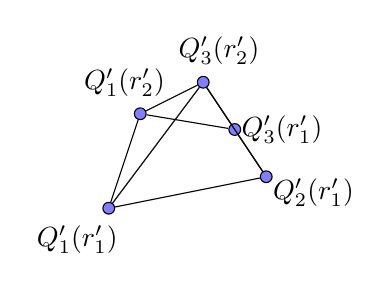
\begin{tikzpicture}[scale=2]

    % Vertices (represent quora points for one replica)
    \node[draw, circle, fill=blue!50, inner sep=1.5pt] (v1) at (0,0) {};
    \node[draw, circle, fill=blue!50, inner sep=1.5pt] (v2) at (1,0.2) {};
    \node[draw, circle, fill=blue!50, inner sep=1.5pt] (v3) at (0.6,0.8) {};
    \node[draw, circle, fill=blue!50, inner sep=1.5pt] (v4) at (0.2,0.6) {};
    \node[draw, circle, fill=blue!50, inner sep=1.5pt] (v5) at (0.8,0.5) {};

    % Edges (1-simplices)
    \draw (v1) -- (v2);
    \draw (v1) -- (v3);
    \draw (v1) -- (v4);
    \draw (v2) -- (v3);
    \draw (v2) -- (v5);
    \draw (v3) -- (v4);
    \draw (v3) -- (v5);
    \draw (v4) -- (v5);

    % Filled triangle (2-simplex)
    \filldraw[fill=green!30, opacity=0.4] (v1) -- (v3) -- (v4) -- cycle;
    \filldraw[fill=yellow!30, opacity=0.4] (v2) -- (v3) -- (v5) -- cycle;

    % Labels (optional)
    \node at (-0.2,-0.2) {$Q'_1(r'_1)$};
    \node at (1.3,0.1) {$Q'_2(r'_1)$};
    \node at (0.7,1.0) {$Q'_3(r'_2)$};
    \node at (0.1,0.8) {$Q'_1(r'_2)$};
    \node at (1.1,0.5) {$Q'_3(r'_1)$};

  \end{tikzpicture}
  \caption{A simplicial complex representing the data of $B$ for three replicas on state transitions $r'_1$ and $r'_2$.}
  \label{fig:simplicial_complex}
\end{figure}


\section{Byzantine Fault Allowing}
We define the category Byzantine Fault Allowing, denoted $\bfa$, as the category of fault-tolerant parametric state machine replica protocols. In the proceeding subsections, we first re-examine our approximations of $B$ as categorical constructions. We then generalize to provide the definition of $\bfa$. Finally, we identify additional elementary constructions which will be leveraged in the section on constructions and implementations.

\subsection{Combinatorial Morphisms and the Fixed Point $B$}

For the sake of exposition, let $\mathcal{D} \hookrightarrow \bfa$ represent a subcategory of $\bfa$ s.t. $\mathrm{Ob}(\mathcal{D})$ represent resampling parameterizations of $B$ described in the previous section. We will formalize $\mathcal{D}$ later.

Assume also any algorithm $A$ which produces quora $Q_B(r') \subseteq Q_A(r')$ is equivalent to $B$.

We can describe a morphism $\mathcal{d}: \mathrm{Ob}(\mathcal{D}) \to \mathrm{Ob}(\mathcal{D})$ which takes a resampling algorithm $X_{k,f}$ using the resampling parameters $k$ and $f$ and increments $k$ by 1. That is...

\begin{flalign*}
  &\mathcal{d}: \mathrm{Ob}(\mathcal{D}) \to \mathrm{Ob}(\mathcal{D}) \\
  &\mathcal{d}(X_{k,f}) = X_{k+1,f} \\
\end{flalign*}

This implies that after $f-k$ such morphisms, we will have produced the algorithm $X_{f,f}$ which is equivalent to $B$. Further application of $\mathcal{d}$ will yield the algorithm $X_{f+1,f}$ which is also equivalent to $B$. This implies that $B = X_{f,f}$ is a fixed point of $\mathcal{D}$ in the category $\bfa$.

\[
\begin{tikzcd}[row sep=2em, column sep=3em]
  X_{k,f} \in \mathcal{D} \arrow[r, "\mathcal{d}"] & \cdots f-k \cdots \arrow[r, "\mathcal{d}"] & B \arrow[loop right, "\mathcal{d}"] \\
  X_{f-1,f} \in \mathcal{D} \arrow[urr, "\mathcal{d}"] &
\end{tikzcd}
\]

\subsection{Definition}
We define $\bfa$ as the permissive category of all subcategories $\mathcal{X} \hookrightarrow \bfa$ which have a fixed point $B$ in the category $\bfa$ together with a fixed point $\mathcal{U}_{\mathcal{X}}$ which indicates the point at which the behavior of the object in the subcategory is no longer defined. 

Diagrammatically, we can represent this as:

\[
\begin{tikzcd}[row sep=2em, column sep=3em]
  X_{k,f} \in \mathcal{D} \arrow[r, "\mathcal{d}"] & \cdots f-k \cdots \arrow[r, "\mathcal{d}"] & B \arrow[loop right, "\mathcal{d}"] \\
\end{tikzcd}
\]

Accordingly, the combinatorial algorithms $X_{k,f}$ and the morphisms $\mathcal{d}$ and $\mathcal{d'}$ in $\mathcal{D}$ are in $\bfa$. Likewise, the topological algorithms $Y_{k,f}$ and their morphisms $\mathcal{t}$ and $\mathcal{t'}$ in $\mathcal{Tt}$ are in $\bfa$. In the following section, we discuss additional constructions within $\bfa$.

\section{Constructions and Implementations}

\section{Conclusion}

%%
%% The acknowledgments section is defined using the "acks" environment
%% (and NOT an unnumbered section). This ensures the proper
%% identification of the section in the article metadata, and the
%% consistent spelling of the heading.
\begin{acks}

\end{acks}

%%
%% The next two lines define the bibliography style to be used, and
%% the bibliography file.
\bibliographystyle{ACM-Reference-Format}
\bibliography{sample-base}


%%
%% If your work has an appendix, this is the place to put it.
\appendix

\end{document}
\endinput
%%
%% End of file `sample-manuscript.tex'.
